%============================ PORTADA =======================================
% Carátula institucional con el mismo diseño Faceta utilizado en el manual.
\begin{titlepage}
\thispagestyle{empty}
\begin{tikzpicture}[remember picture,overlay]
  \coordinate (NW) at (current page.north west);
  \node[anchor=north west,inner sep=0] at (NW)
    {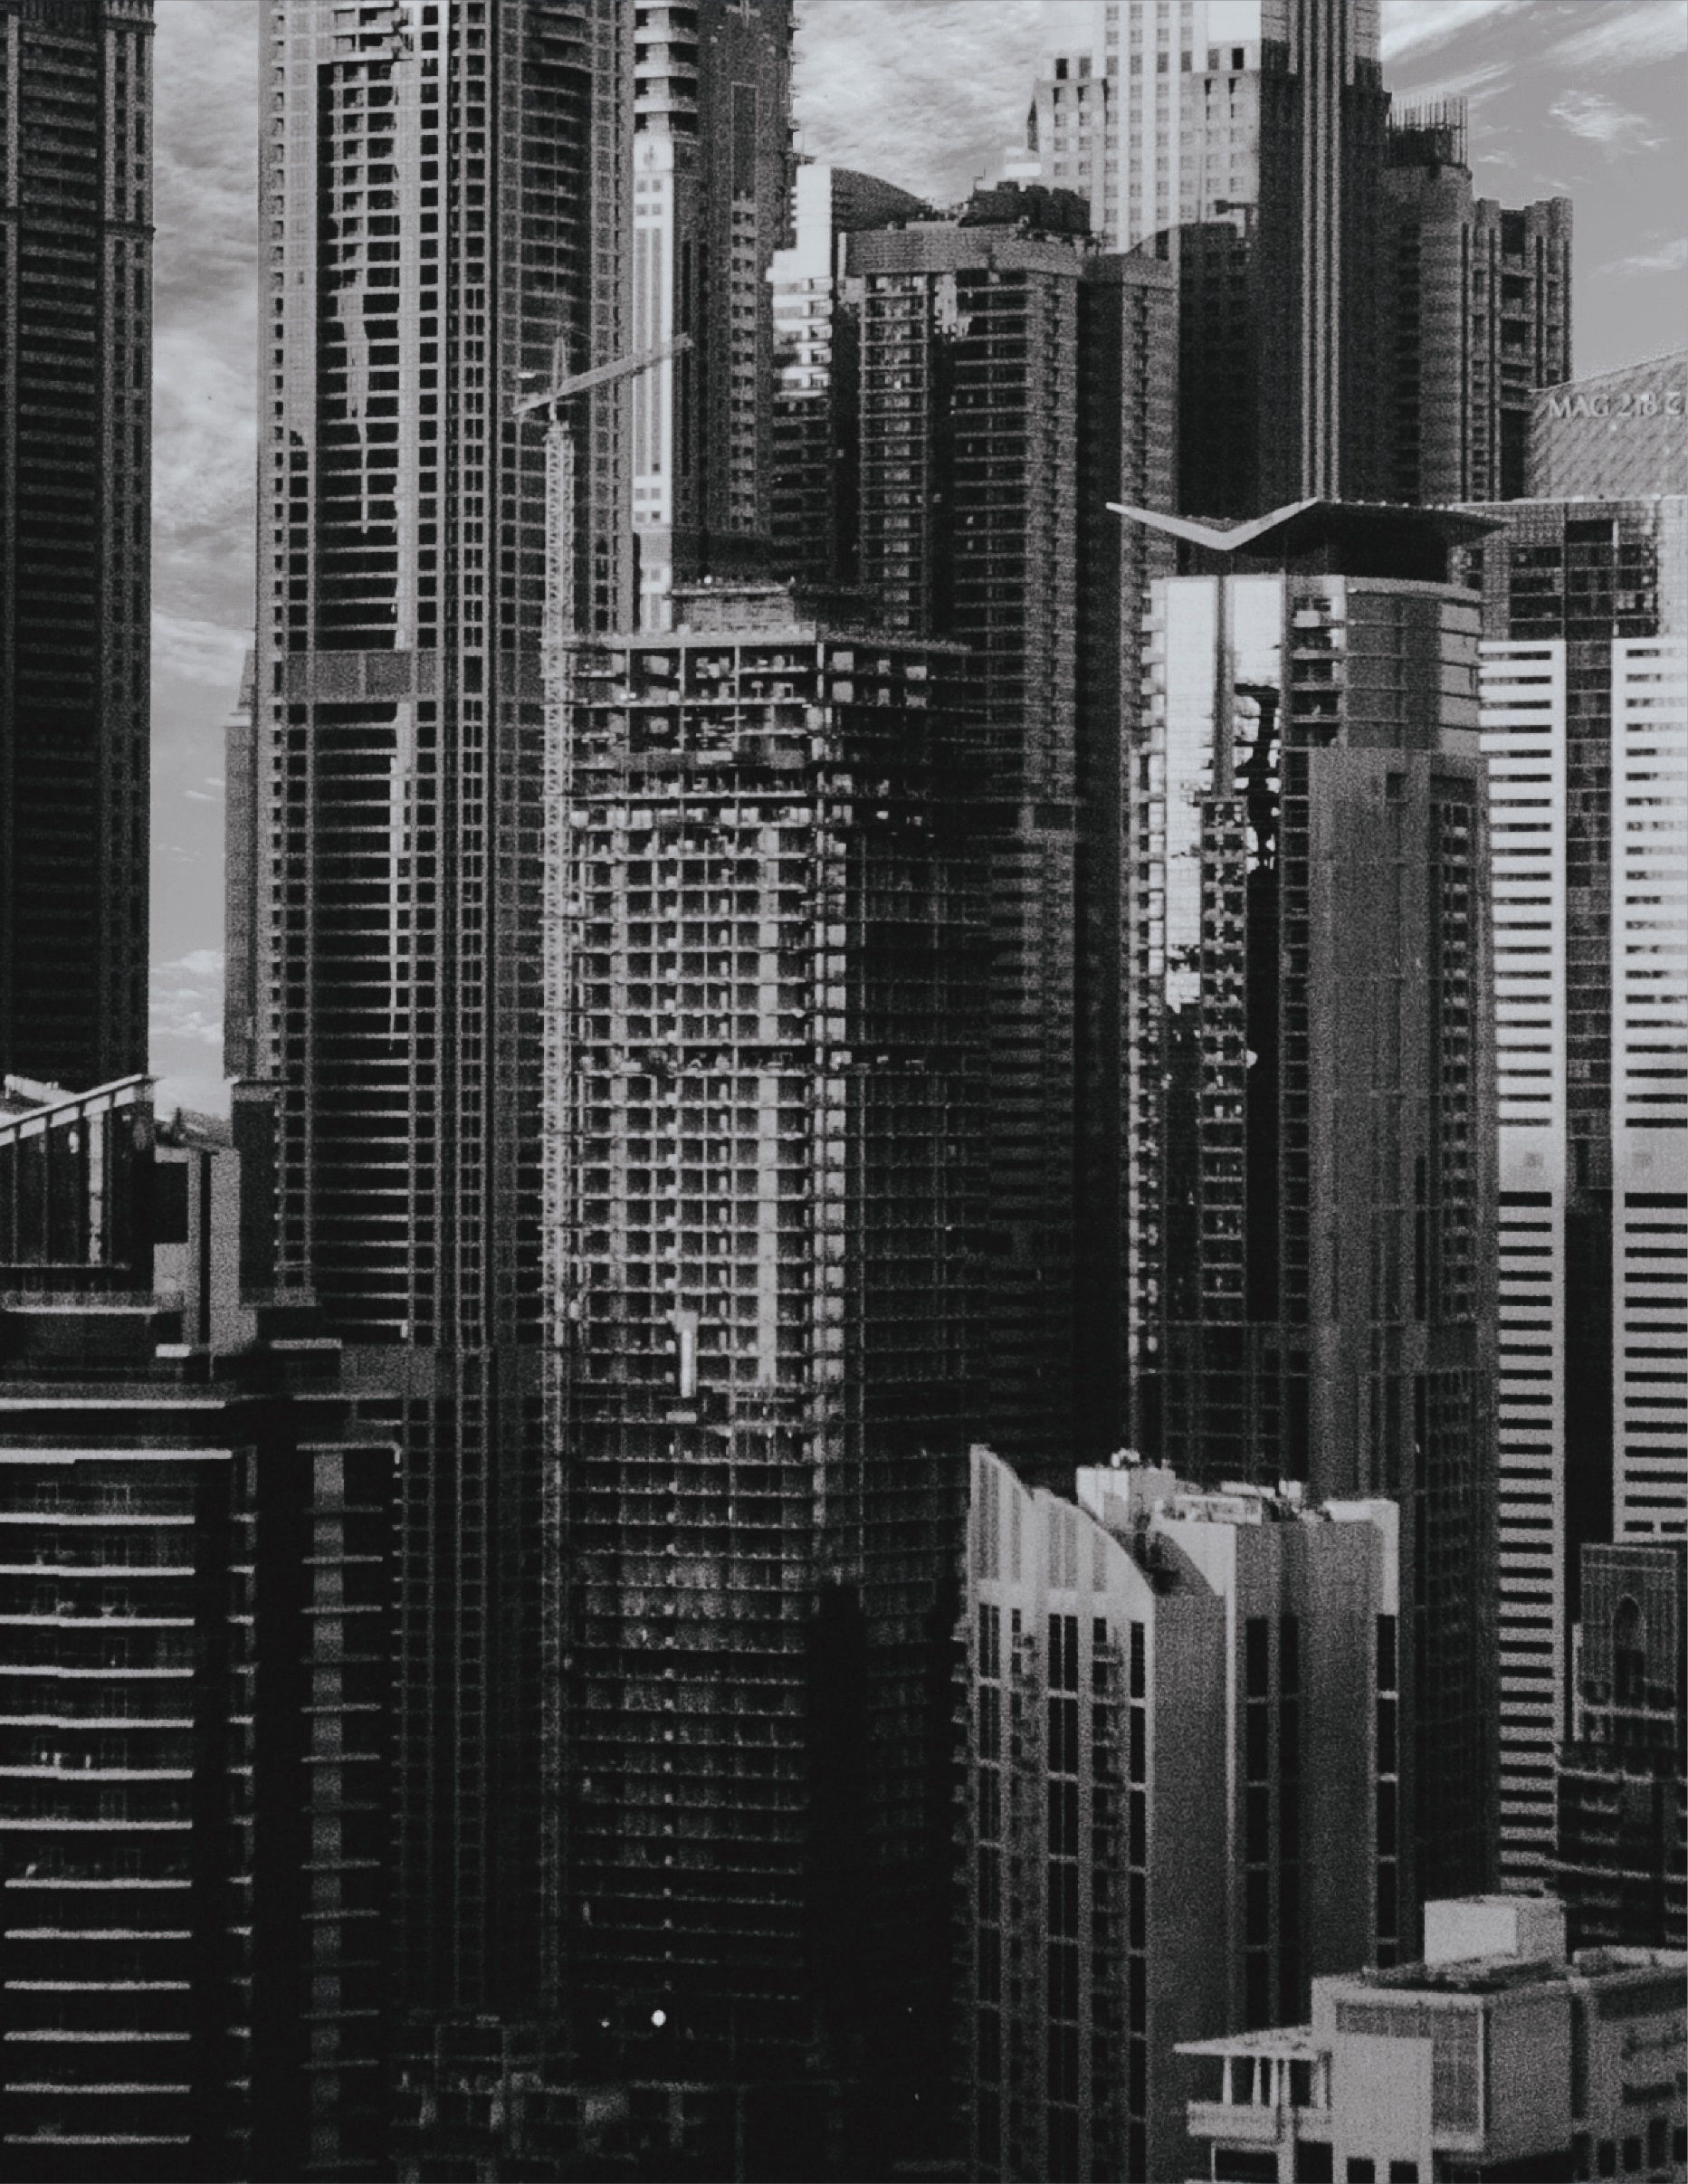
\includegraphics[width=\paperwidth,height=\paperheight]{figuras/portada-ciudad}};
  \fill[facetgreen] ([yshift=-18mm]NW) rectangle ([xshift=9mm,yshift=-95mm]NW);
  \node[anchor=north west,text=white,align=left,font=\sffamily\bfseries\large]
    at ([xshift=16mm,yshift=-24mm]NW) {PROYECTO TECNOLÓGICO};
  \node[anchor=north west,text=white,align=left,font=\sffamily\small]
    at ([xshift=16mm,yshift=-33mm]NW)
    {Desarrollo en Sistemas de Información y Ciberseguridad};
  \fill[facetred,opacity=0.95]
    ([yshift=-142mm]NW) rectangle ([xshift=\paperwidth,yshift=-214mm]NW);
  \node[anchor=west,text=white,align=left,text width=175mm,font=\sffamily]
    at ([xshift=17mm,yshift=-177mm]NW)
    {{\fontsize{15}{17}\selectfont EILOR}\\[4pt]
     {\fontsize{29}{33}\selectfont\bfseries Analizador táctico de espectro}\\[-1pt]
     {\fontsize{29}{33}\selectfont\bfseries 2.4\,GHz, radar BLE y portal de registro}\\[6pt]
     {\fontsize{11}{13}\selectfont\itshape Sistema basado en ESP32, Node.js y WebSocket en tiempo real}};
  \fill[facetnavy] ([yshift=-214mm]NW) rectangle ([xshift=\paperwidth,yshift=-241mm]NW);
  \node[anchor=west,text=white,align=left,text width=175mm,font=\sffamily\bfseries]
    at ([xshift=17mm,yshift=-227.5mm]NW)
    {DESARROLLO DE PROYECTO TECNOLÓGICO EN SISTEMAS DE INFORMACIÓN Y CIBERSEGURIDAD};
  \fill[white,opacity=0.92] ([yshift=-241mm]NW) rectangle ([xshift=\paperwidth,yshift=-297mm]NW);
  \node[anchor=north west,text=facetdark,align=left,font=\sffamily,text width=120mm]
    at ([xshift=17mm,yshift=-247mm]NW)
    {\textbf{\color{facetred}Autor}\\[2pt]
     Pablo Alejandro Tandazo Zarango\\
     \textbf{Tutor / docente}\\[2pt]
     Ing. Marco Silva, Mg};
  \node[anchor=south east,inner sep=0] at ([xshift=\paperwidth-16mm,yshift=-289mm]NW)
    {
\includegraphics[width=52mm]{figuras/logo-sic}};
  \node[anchor=south west,text=facetnavy,font=\sffamily\small\bfseries]
    at ([xshift=17mm,yshift=-286mm]NW) {Ciudad, provincia};
  \node[anchor=south west,text=facetnavy,font=\sffamily\small\bfseries]
    at ([xshift=17mm,yshift=-292mm]NW) {\today};
\end{tikzpicture}
\end{titlepage}
